\chapter{Úvod}
\blindtext

Cílem této bakalářské práce je vytvořit webovou aplikaci typu Kanban určenou pro řízení projektů na základě požadavků společnosti SEACOMP s.r.o. Za tímto účelem je společností v současné době využíván nástroj třetí strany, který ovšem není plně přizpůsoben potřebám této společnosti, ku příkladu není integrován do dalších interních aplikací.

Téma práce mne zaujalo zejména díky stále rostoucí popularitě interaktivních webových aplikací, motivující pro mne bylo mít možnost takovou aplikaci implementovat naprosto sám. Také mne lákala možnost firemního zadání bakalářské práce, díky kterému bude mít výsledná aplikace reálné využití a bude využívána v praxi. 

\blindtext

Druhá kapitola práce, zvaná \uv{Rozbor řešené problematiky}, pojednává o historii a současných trendech projektového řízení, zejména pak o metodice Kanban. Poté následuje přehled několika nástrojů určených pro aplikaci této metodiky a jejich srovnání.
Dále je pár slov věnováno zadavateli této diplomové práce -- společnosti SEACOMP s.r.o., infrastruktuře této společnosti a požadavkům na výslednou aplikaci.
Další kapitola, označená \uv{Technologie}, obsahuje stručný přehled technologií a principů využitých při implementaci této aplikace.
Následující kapitola s názvem \uv{Návrh aplikace} % @todo
Pátá kapitola jménem \uv{Implementace aplikace}, se pak věnuje zajímavým částem řešení této bakalářské práce. 
Kapitola \uv{Testování a vyhodnocení} % @todo
Na závěr je poté shrnuto % @todo



\chapter{Rozbor řešené problematiky}
V úvodu této kapitoly jsou stručně shrnuty populární metodiky řízení projektů s větším zaměřením na metodiky agilní a to především na metodiku Kanban. V další části kapitoly je představeno několik již existujících aplikací umožňujících využívat právě tuto zmíněnou metodiku. Dále je text věnován zmapování infrastruktury zadavatele bakalářské práce a jeho požadavkům na výslednou aplikaci. Závěr kapitoly obsahuje popis technologií, které byly využity pro tvorbu požadované aplikace.

\section{Metodiky řízení projektů}
Obecně lze metodiky používané pro řízení softwarových projektů rozdělit do dvou hlavních kategorií. Jedná se o tradiční metodiky a metodiky agilní.

Jak název napovídá, tradiční metodiky mají delší historii. Lidstvo potřebovalo využívat řízení projektů již odpradávna, exemplárním příkladem jsou obrovské stavební projekty jako pyramidy v Gíze nebo Velká čínská zeď. Tyto projekty jistě vyžadovaly důkladné řízení jak pracovních sil, tak i přísunu materiálu a dalších zdrojů. Výsledek musel bezpochyby splňovat určité požadavky. Ohledně metodik takovýchto plánování ovšem neexistuje příliš mnoho dokumentace. K určité standardizaci řízení projektů totiž začalo docházet až v padesátých letech minulého století. Svou zásluhu zde má i Námořnictvo Spojených států amerických a to konkrétně Projekt Manhattan\footnote{Krycí název pro projekt vývoje atomové bomby během druhé světové války}~\cite{bib:project-managment-history}.

Rozdílem mezi dvěma zmíněnými kategoriemi řízení projektů je především strukturace procesů. U tradičních metod probíhají tyto procesy sekvenčně. Tento přístup zpravidla vyžaduje důkladnější počáteční plánování a pozdější změny požadavků mnohdy představují náročný problém. Oproti tomu při použití agilních metod jsou jednotlivé procesy úzce spjaty a pracuje se v iteracích. Díky tomu je do vývoje více zapojen zákazník a takovýto projekt se snadněji vypořádá s případnými změnami požadavků~\cite{bib:agile-vs-traditional}. 

Populárním zástupcem tradičních metodik je například vodopádový model (znázorněný diagramem~\ref{img:waterfall}), na kterém je na první pohled patrné právě sekvenční řazení jednotlivých procesů vývoje. Tento model se objevil koncem šedesátých let minulého století, kdy byly programovací jazyky neefektivní, procesory pomalé a paměť počítačů byla výrazně omezená~\cite{bib:agile-history}. 

\begin{figure}[H]
	\centering
	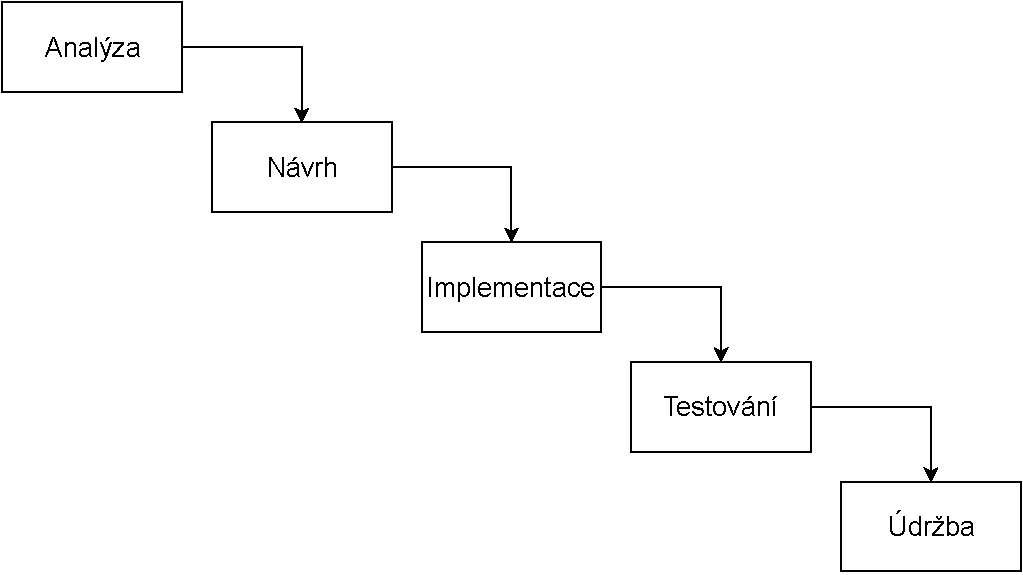
\includegraphics[width=0.8\textwidth]{obrazky-figures/waterfall-wide.pdf}
	\caption{Grafické znázornění posloupnosti jednotlivých procesů tradiční metodiky řízení projektů označované jako vodopádový model.}
	\label{img:waterfall}
\end{figure}

U tradičních metodik je předpokladem, že se k dokončeným fázím projektu již nebude nutné vracet. Takový předpoklad lze aplikovat na mnoho odvětví. Příkladem budiž stavba budovy, u které je nutné nejprve řádně celý projekt naplánovat a zdokumentovat. Jakmile samotná stavba započne, větší změny oproti původnímu projektu vznikají velmi zřídka. V oblasti informačních technologií, obzvláště při vývoji softwaru, však odchýlení od původního plánu nebývá žádnou výjimkou. Řízení projektů tohoto typu pomocí striktních tradičních metodik je tedy často obtížné a značně neefektivní~\cite{bib:agile-vs-traditional-what}.

V dnešní době se stává častěji než tomu bylo v minulosti, že se softwarové projekty během vývoje mění, narůstají jejich požadavky, přibývají funkce a to vše i během jejich vývoje. Tento trend se týká především webových systémů. Jako reakce na tyto náhlé změny byly v devadesátých letech stvořeny právě agilní metodiky~\cite{bib:agile-history}. 

\subsection{Agilní metodiky řízení projektů}
Agilní metodiky jsou skupina metod řízení projektů určena především pro vývoj softwaru. Jak název napovídá, jedná se o metodiky, které se vyznačují dynamičností a flexibilitou.

Veřejný zájem o tyto metodiky začal až v pozdních devadesátých letech~\cite{bib:agile-mobile}. V roce 2001 se v Utahu sešlo sedmnáct zastánců agilních metodik a sestavilo Manifest agilního vývoje software\footnote{ Manifest agilního vývoje: \url{https://agilemanifesto.org/iso/cs/manifesto.html}}, který vystihuje čtyři hlavní zásady těchto metod~\cite{bib:agile-manifest}.
\begin{itemize}
  \item Jednotlivci a interakce před procesy a nástroji
  \item Fungující software před vyčerpávající dokumentací
  \item Spolupráce se zákazníkem před vyjednáváním o smlouvě
  \item Reagování na změny před dodržováním plánu
\end{itemize}

Tyto metodiky jsou více zaměřené na lidi a na jejich vzájemnou komunikaci. To je jedním z důvodů, proč jsou agilní metodiky vhodné především pro menší týmy. Díky absenci sekvenčního řazení procesů vývoje tyto metody také zvyšují efektivitu nepředvídatelných a stále se měnících projektů. Vypuštěním striktního plánování je také možné projekt mnohdy dokončit rychleji než použitím tradičních metodik.

Vývoj řízený agilními metodikami probíhá iterativně a inkrementálně. Na začátku vývoje se určí základní požadavky a postupnými cykly se tyto požadavky zdokonalují. Jedna iterace takového vývoje trvá zpravidla jeden týden až měsíc. Během této iterace proběhne celý cyklus vývojových procesů (podobný vodopádovému modelu znázorněného diagramem~\ref{img:waterfall}). Dokončením iterace vzniká prototyp, který může být prezentován zákazníkovi. Díky tomu zákazník získává přesnější představu o podobě produktu a lze včas odhalit nedostatky požadavků, které dříve nebyly známy~\cite{bib:agile-impact}. 
Průběh tohoto iterativního vývoje je znázorněný diagramem~\ref{img:agile}.

\begin{figure}[H]
	\centering
	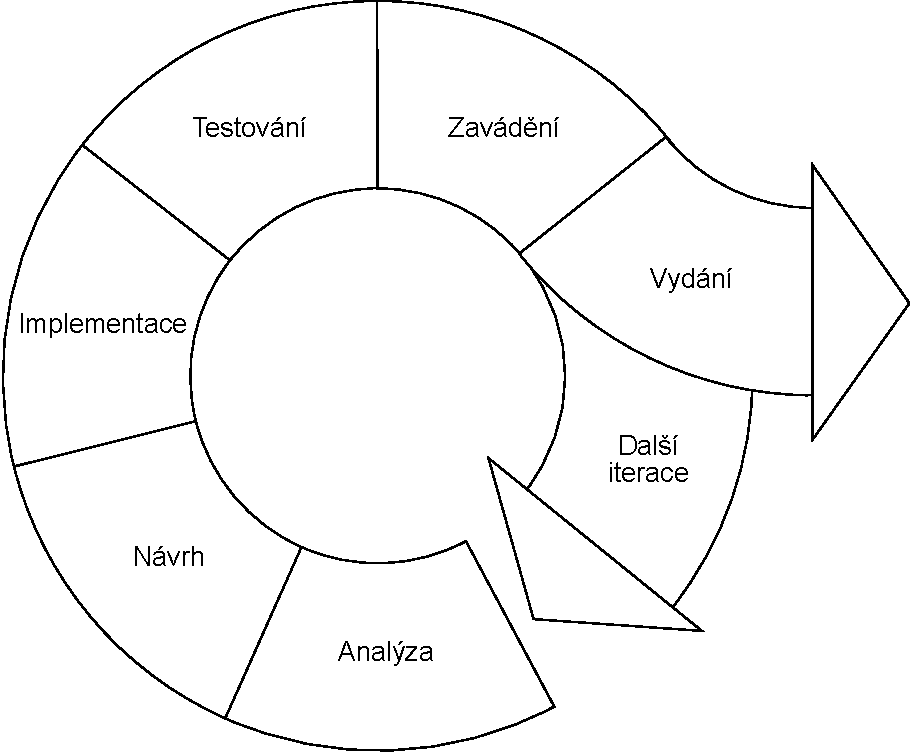
\includegraphics[width=0.7\textwidth]{obrazky-figures/agile.pdf}
	\caption{Grafické znázornění posloupnosti jednotlivých procesů agilních metodik řízení projektů. Cyklus začíná procesem analýza a pokračuje až po proces zavádění, kdy je projekt buďto hotov a následuje jeho vydaní nebo proběhne další iterace a celý cyklus se znovu opakuje.}
	\label{img:agile}
\end{figure}

Mezi populární agilní metodiky patří například Scrum, Lean Developmet, Extrémní programování (angl. \emph{Extreme Programming} nebo také XP), Crystal, Vlastnostmi řízený vývoj (angl. \emph{Feature Driven Development} neboli FDD) a v neposlední řadě také Kanban.

Jedna ze studií na toto téma vydána roku 2015 uvádí, že ze 1386 sledovaných projektů 65\% z nich využilo během vývoje agilní metody a 6\% projektů bylo dokončeno téměř pouze s použití agilních metod. Závěrem této studie je také pozorování poukazující na fakt, že čím větší poměr agilních metodik byl při vývoji použit, tím úspěšnější dané projekty byly~\cite{bib:agile-work}.

\subsection{Metodika Kanban}
Kanban je slovo převzaté z japonského jazyka, kde znamená \uv{cedule}. Toto slovo je taktéž spjato s poslední výzvou k objednávce před uzavřením podniku (sundáním cedule). Takovou objednávku lze označit jako \uv{na poslední chvíli} nebo také jako objednávku \uv{tak akorát na čas}~\cite{bib:dict-kanban}. 

Tak akorát na čas (anglicky \emph{Just-in-time}) je filozofie řízení výroby, vyvinuta v sedmdesátých létech japonskou automobilovou společností Toyota Motor Corporation\footnote{Toyota Motor Corporation: \url{https://global.toyota/en/}}. Hlavní myšlenkou toho přístupu je mít přesné množství materiálu, na správném místě a ve správný čas. Díky tomu dochází k redukci množství materiálu, který aktuálně není zpracováván a nemělo by docházet k jeho přebytečnému hromadění~\cite{bib:just-in-time}. Jedním z nástrojů této filozofie je právě metodika Kanban, její tehdejší provedení je možné vidět na fotografii~\ref{img:kanban-toyota}.

\begin{figure}[H]
	\centering
	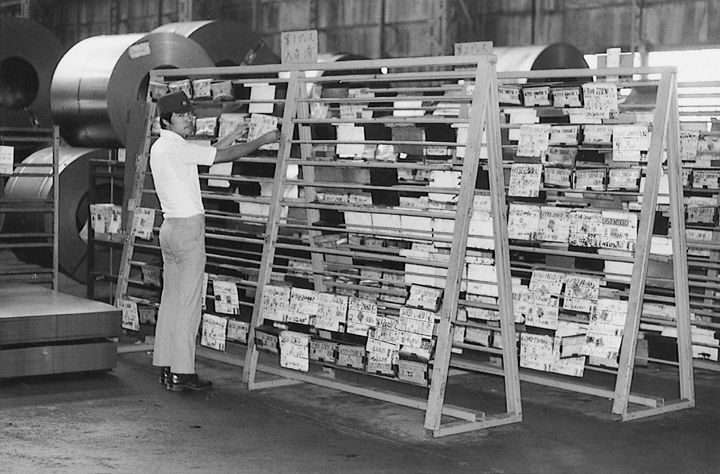
\includegraphics[width=\textwidth]{obrazky-figures/toyota-kanban.jpg}
	\caption{Původní provedení kanbanu v továrně společnosti Toyota Motor Corporation \emph{Převzato z~\cite{bib:toyota-history}}.}
	\label{img:kanban-toyota}
\end{figure}

Metodika Kanban je nástroj pro vizuální kontrolu práce a jejího toku jednotlivými fázemi procesu. Kanban může být realizován jak fyzicky (například tabule s nalepovacími papírky viz fotografie~\ref{img:kanban-whiteboard}), tak i digitálně (například pomocí aplikací uvedených v kapitole~\ref{sec:apps}). 

Ať je nástěnka Kanban digitální či nikoliv, ve většina případů se skládá ze stejných částí, jen v jiném provedení. Nejčastěji se lze setkat s typem, kdy na se na horizontální ose nachází pojmenované sloupce představující jednotlivé fáze procesu. Do těchto sloupců jsou umístěny nejrůznější karty, reprezentující jednotlivé úkoly. Rozmístění karet mezi sloupci se odvíjí od aktuálního stavu úkolu.

Nejjednodušší variantou takových sloupců může být například trojce sloupců nazvaných \uv{zásobník}, \uv{v procesu} a \uv{hotovo}. První ze sloupců nazvaný \uv{zásobník} je místo, kde se hromadí úkoly, na kterých se ještě nezačalo pracovat. Jakmile práce na daném úkolu započne, jeho karta je přesunuta do dalšího sloupce s označením \uv{v procesu}. Obdobně je tomu při dokončení úkolu, kdy je jeho karta opět přemístěna do jiného sloupce, tentokrát do sloupce \uv{hotovo}. Názorná ukázka této nástěnky je vidět na fotografii~\ref{img:kanban-whiteboard}.

\begin{figure}[H]
	\centering
	
\includegraphics[width=\textwidth]{obrazky-figures/placeholder.pdf}
	\caption{Nástěnka typu Kanban realizována pomocí nalepovacích papírků na magnetické tabuli.}
	\label{img:kanban-whiteboard}
\end{figure}

V praxi je takřka nemožné setkat se s takto jednoduchým provedením. Proces výroby či vývoje je třeba rozdělit na jednotlivé části. Při vývoji softwaru bývají často využívány sloupce \uv{návrh}, \uv{vývoj}, \uv{testování} a další.  

Pokud jednu nástěnku využívá více oddělení společnosti, lze se mnohdy setkat i s dalším rozlišením úkolů. Jedná se o takzvané plavecké dráhy (angl. swimlanes). Úkoly jsou pak rozděleny nejen do sloupců (značících procesy), ale i do vodorovných řádků, které nejčastěji představují jednotlivá oddělení společnosti či týmy. 

V dnešní době, jak u mnoha věcí, převažuje digitální provedení Kanban nástěnek. Její výhodou je především větší přehlednost, vzdálená přístupnost, jednoduší manipulace a hlavně možnost připojovat k jednotlivým kartám podrobnější popis, komentáře, obrázky a další dokumenty. Nicméně i fyzická varianta má své výhody. Jedna z nich je fakt, že je stále na očích a nelze ji skrýt jako například záložku v prohlížeči. Toto provedení může taktéž podněcovat k vetší komunikaci mezi týmy a to jsou důvody proč tuto variantu využívají například ve společnosti Optimizely\footnote{Optimizely: \url{https://www.optimizely.com/about/}}~\cite{bib:kanban-atlassian}.

Díky využití metodiky Kanban a jejího přehlednému vyobrazení úkolů získávají jednotliví členové týmu lepší přehled o prací svých kolegů. Tento fakt může také vést k lepší prioritizaci úkolů a především odpadá čas ztracený komunikací v momentě kdy nastane změna úkolu čí jeho priority~\cite{bib:kanban-101}.
Kanban svou podstatou také dokáže poukázat na problematické procesy, které zpomalují celkový chod výroby či vývoje~\cite{bib:kanban-and-scrum}.

Často se u metodiky Kanban lze potkat s limitováním probíhající práce (anglicky \emph{Work in Progress]} či zkráceně WIP). Jedná se o omezení, kdy dán maximální počet úkolů pro určitou fázi procesu (sloupec nástěnky). Například lze stanovit limit souběžného pracování maximálně na třech grafických návrzích. Toto omezení má pozitivní dopad především na snížení nutnosti věnovat se více projektům naráz, díky čemuž se lze na jednotlivé úkoly lépe soustředit a tím může být docíleno rychlejšího a kvalitnějšího výsledku~\cite{bib:kanban-101}.

\section{Aplikace s podobným zaměřením}\label{sec:apps}
Jelikož metodika Kanban existuje již několik několik desítek let, lze v dnešní době nalézt celou řadu programů a webových aplikací, které je možné pro aplikování této metodiky využít. V této podkapitole je několik takových aplikací stručně přiblíženo a jsou vyzdviženy některé jejich klíčové vlastnosti. Pro bližší představu o podobě těchto aplikací je každá doprovázena jejím snímkem. Mezi uvedenými aplikacemi lze nalézt dva populární zástupce z řad produktů společnosti Atlassian -- aplikace Trello a Jira. Třetí představenou aplikací je o něco méně známá aplikace Kanboard, která je však v současné době využívaná společností SEACOMP s.r.o. V závěru kapitoly je obsaženo stručné shrnutí rozdílů těchto tří aplikací a možné důvody vedoucí ke zvolení právě jedné z uvedených aplikací.

\subsection{Trello}
Trello\footnote{Trello: \url{https://trello.com}} je především webová aplikace provozovaná v současné době společností Atlassian\footnote{Atlassian: \url{https://www.atlassian.com}}. Historie této aplikace sahá až do roku 2011, kdy byla veřejně spuštěna jako webová aplikace a také jako aplikace pro platformu iOS. K dnešnímu dni je aplikaci Trello možné navíc využít i na mobilní platformě Android nebo jako desktopová aplikace pro operační systémy Microsoft Windows či macOS. 

Během několika let své existence se aplikace stala velice populární a použilo ji několik milionů uživatelů. K věhlasným společnostem, které tuto aplikaci využívají patří například technologický gigant Google\footnote{Google: \url{https://about.google/}}, softwarová společnost Red Hat\footnote{RedHat: \url{https://www.redhat.com/en/about/company}} nebo platforma pro skupinové financování Kickstarter\footnote{Atlassian: \url{https://www.kickstarter.com/about}}~\cite{bib:trello-about}. 

Svou velkou popularitu si aplikace zasloužila především přívětivým uživatelským rozhraním a jednoduchostí použití. Od první návštěvy stránky k práci na své první Kanban nástěnce uživatele dělí doslova minuty. Pro základní použití navíc bez problému vystačí bezplatná verze aplikace. Díky těmto faktům aplikace není využívána pouze softwarovými společnostmi, ale lze ji použít například i jako osobní seznam úkolů~\cite{bib:jira-vs-trello}.

Trello nabízí řadu vylepšení, díky kterým je možné nástěnku rozšířit o funkce z aplikací třetích stran. 
V bezplatné verzi lze však využít pouze jedno takové vylepšení~\cite{bib:trello-pricing}.
Nástěnka je umístěna na vzdáleném úložišti a službu nelze provozovat na svém vlastním serveru. Nicméně mobilní aplikace umožňují pracovat s nástěnkami i bez přístupu k internetu~\cite{bib:trello-common}.

\begin{figure}[H]
	\centering
	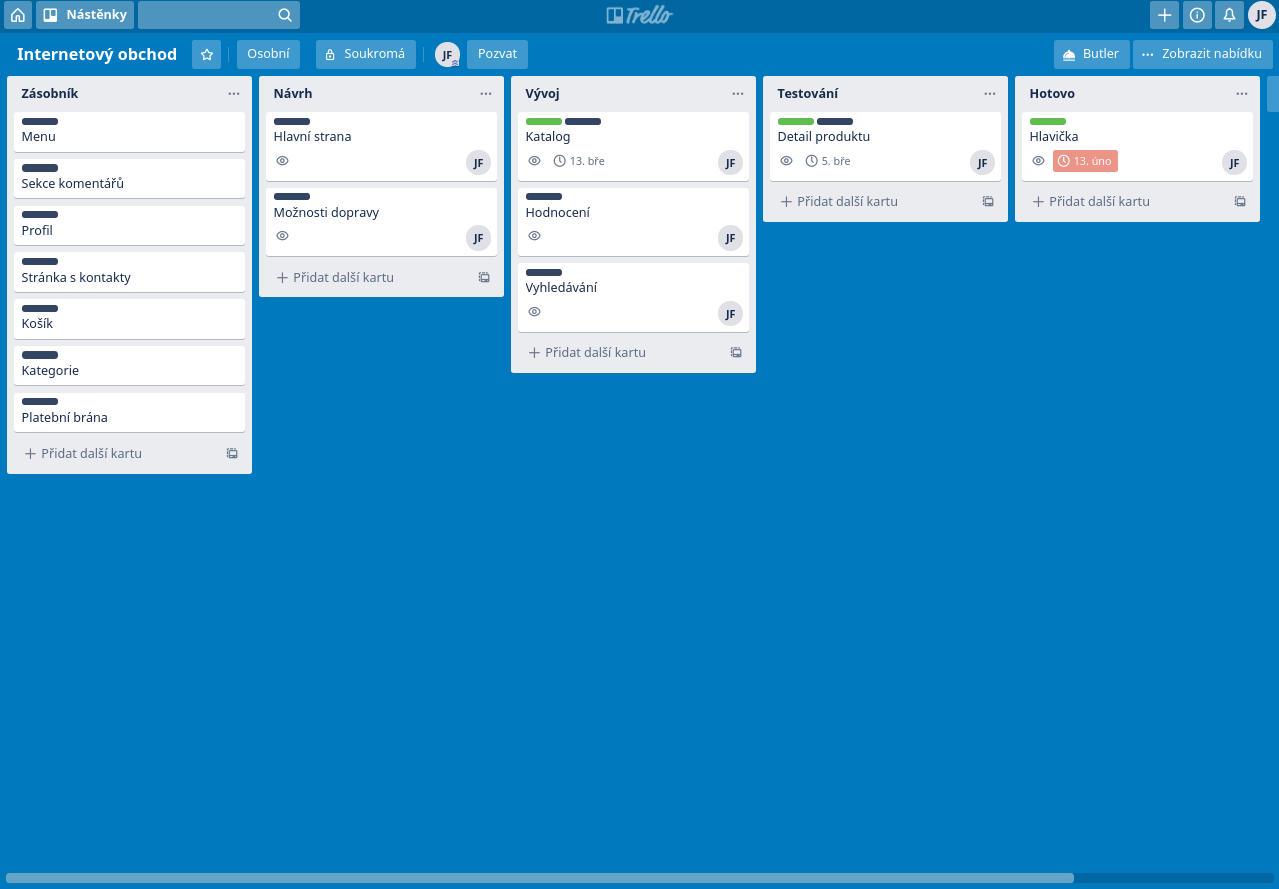
\includegraphics[width=\textwidth]{obrazky-figures/trello.png}
	\caption{Vzorová Kanban nástěnka ve webové aplikaci Trello zaměřená na vývoj internetového obchodu.}
\end{figure}

\subsection{Jira}
Jira\footnote{Jira: \url{https://www.atlassian.com/cs/software/jira}} je řada produktů společnosti Atlassian, určená ke správě práce v nejrůznějších typech týmů. Nástěnka Kanban je součást například produktu Jira Software, který je, jak název vypovídá, zaměřen především na vývojáře softwaru. 
% https://www.atlassian.com/software/jira/guides/getting-started/overview#jira-software-hosting-options

S nástěnkou lze pracovat jak v prohlížeči, tak i pomocí vlastního programu, který je k dispozici pro operační systémy Microsoft Windows, Linux i macOS. K dispozici jsou také mobilní aplikace pro operační systém iOS i Android. 

Jednou z funkcí, kterou Jira disponuje, je možnost vygenerování řady grafů a přehledů. V základní verzi bez přídavných modulů lze také tvořit dílčí úkoly a vzájemné závislosti jednotlivých úkolů. Základní funkcionalitu aplikace lze rozšířit využitím placených i bezplatných doplňku, které jsou k dispozici na oficiálním tržišti.

Díky tomu, že je aplikace určená pro softwarové vývojáře je v této aplikaci mimo klasické nástěnky možné také přepnout režim zobrazení na variantu určenou pro agilní metodiku zvanou Scrum, která cílí na dokončení úkolů v rámci iterace cyklu vývoje~\cite{bib:trello-vs-jira-2020}.

Nástěnka může být na rozdíl od aplikace Trello umístěna jak na vzdáleném úložišti, tak na vlastním serveru.

Tato aplikace je využívána více něž 65 tisíci zákazníky po celém světě mezi které se řadí například internetovou aukční síň eBay\footnote{eBay: \url{https://www.ebayinc.com/company/}}, služba pro streamování hudby Spotify\footnote{Spotify: \url{https://newsroom.spotify.com/company-info/}}, společnost vyrabějící síťové prvky Cisco\footnote{Cisco: \url{https://www.cisco.com/c/en_uk/index.html}} nebo aplikace pro pronájem ubytování Airbnb\footnote{Airbnb: \url{https://news.airbnb.com/about-us/}}~\cite{bib:jira-homepage}.

\begin{figure}[H]
	\centering
	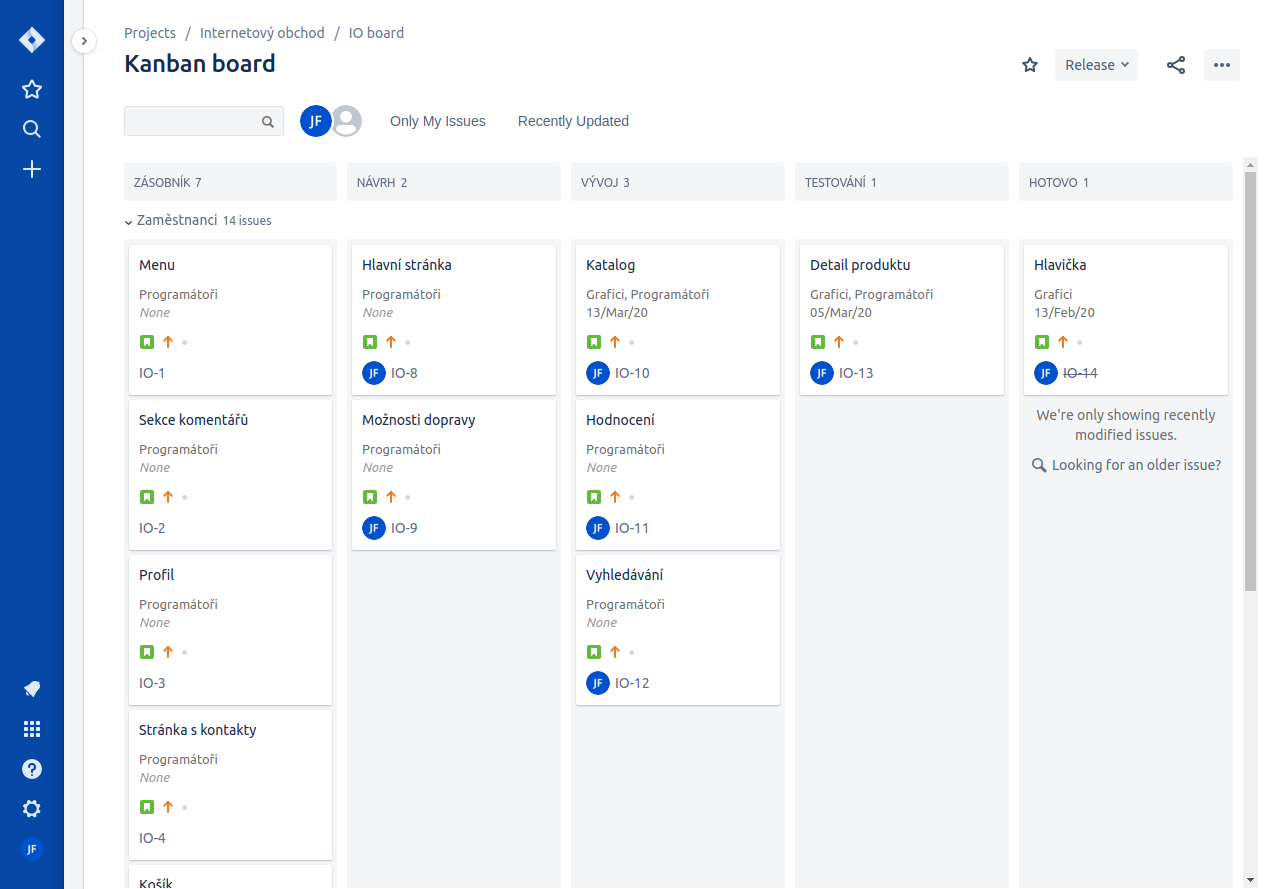
\includegraphics[width=\textwidth]{obrazky-figures/jira.png}
	\caption{Vzorová Kanban nástěnka ve webové aplikaci Jira Software zaměřená na vývoj internetového obchodu.}
\end{figure}

\subsection{Kanboard}
Kanboard\footnote{Kanboard: \url{https://kanboard.org}} je bezplatná webová aplikace s otevřeným zdrojovým kódem. Jejím tvůrcem je Frédéric Guillot, nicméně zdrojové kódy jsou volně k dispozici na portálu GitHub\footnote{Repozitář Kanboard na platformě GitHub: \url{https://github.com/kanboard/kanboard}}, kde se k vývoji připojilo dalších 270 lidí~\cite{bib:kanboard-github}. Aplikace je napsaná především v jazyce PHP a JavaScript. K provozování této aplikace je nutné použít vlastní webový server. Kanboard uživatelům nenabízí žádné přepychové uživatelské rozhraní, ale naopak se zaměřuje na jednoduchost a minimalismus~\cite{bib:kanboard}.

Mimo základní funkce metodiky Kanban tato aplikace umožňuje také vyhledávat úkoly za pomocí vlastního dotazovacího jazyka. Částečně také umožňuje práci s nástěnkou automatizovat pomocí konfigurovatelných akcí.

Vzhledem k otevřenému zdrojovému kódu lze aplikaci v případě potřeby upravit na míru vlastním potřebám. Součástí aplikace je však i rozhraní pro zásuvné moduly. Několik takových modulů lze nalézt i přímo na oficiální stránce\footnote{Zásuvné moduly pro Kanboard: \url{https://kanboard.org/plugins.html}}, avšak nepodléhají žádnému schvalovacímu procesu a není zaručena jejich kompatibilita.

Aplikace však nenabízí žádný program či mobilní aplikaci. Jediný přístup k nástěnce je tedy pomocí internetového prohlížeče.

\begin{figure}[H]
	\centering
	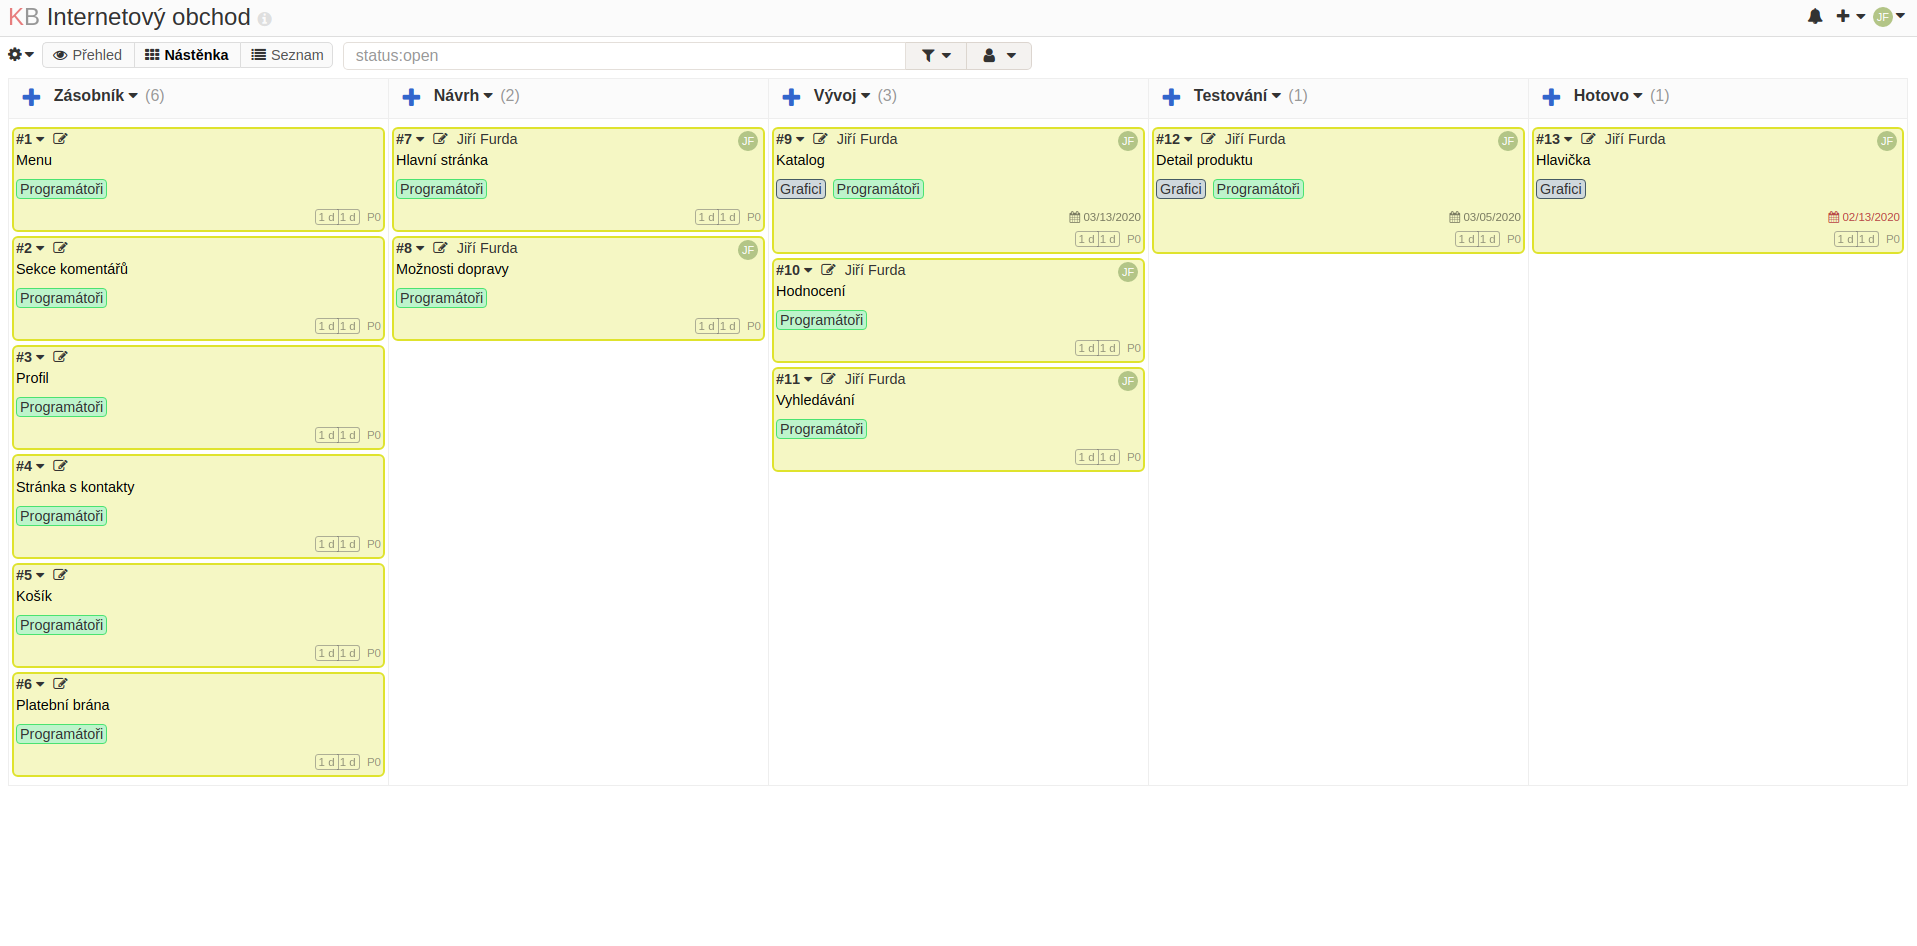
\includegraphics[width=\textwidth]{obrazky-figures/kanboard.png}
	\caption{Vzorová Kanban nástěnka ve webové aplikaci Kanboard zaměřená na vývoj internetového obchodu.}
\end{figure}

\subsection{Souhrn rozdílů}

Základní principy nástěnky Kanban jsou součástí všech tří uvedených aplikací. Malou odchylkou je aplikace Trello, která neumožňuje úkoly rozřadit do plaveckých drah. Této funkcionality lze docílit pouze instalací zásuvného modulu do prohlížeče, což zcela jistě není nejvhodnější řešení.

Představené aplikace se mezi sebou liší například cenou, možnostmi provozování, dostupností zdrojového kódu, existencí mobilní aplikace, dostupností technickou podporou či přívětivostí uživatelského prostředí. Srovnání několik těchto vlastností je přehledně uvedeno v tabulce~\ref{tab:kanban-sum}. 

\begin{table}[hbt]
\centering
\caption{Srovnání rozdílů mezi několika aplikacemi typu Kanban}
\label{tab:kanban-sum}
\begin{tabular}{ |l|c|c|c|c| } 
\hline
Aplikace & Cena\footnotemark & Vzdálené úložiště & Vlastní úložiště & Otevřený zdrojový kód  \\
\hline
Trello & 0--20,83 dolarů~\cite{bib:trello-pricing} & Ano & Ne & Ne \\ 
Jira & 0--14 dolarů~\cite{bib:jira-pricing} & Ano & Ano & Ne \\ 
Kanboard & Zdarma & Ne & Ano & Ano \\ 
\hline
\end{tabular}
\end{table}
\footnotetext{Cena na uživatele za měsíc}

Z důvodu ochrany firemního tajemství mohou být preferovány služby Jira a Kanboard, jelikož je možné je provozovat přímo na svém vlastním serveru. Konkrétně u aplikace Kaboard může tato vlastnost však představovat pro řadu uživatelů nevýhodu. Aplikaci totiž není možné jednoduše provozovat na vzdáleném úložišti. Uživatel musí mít k dispozici server, kde bude aplikace provozována a to se může stát bariérou pro méně pokročilé uživatele počítače.

Kanboard však jako jediná z tří uvedených aplikací disponuje otevřeným zdrojovým kódem. Umožňuje tak větší zásahy do aplikace než je tomu v případě dalších dvou aplikací, kde lze úpravy řešit pouze pomocí doplňků.

Co se ceny týče, všechny aplikace lze provozovat v jistém měřítku zdarma. Trello v bezplatné verzi omezuje počet týmových nástěnek a Jira zase využívá limit uživatelů. Oproti tomu Kanboard, je zcela zdarma. Jediné reálné náklady tedy může představovat provoz serveru. Při provozování aplikace Jira tímto způsobem je třeba uhradit jednorázový poplatek, jehož cena se odvíjí od počtu uživatelů. Použití aplikace Kanboard se tedy může jevit jako nejlepší volba, každopádně v tomto případě je ztracena dostupnost technické podpory. V korporačním prostředí to může být důležitý požadavek, protože výpadek klíčového nástroje pro řízení projektů představuje obrovské riziko pro bezproblémový chod společnosti.

Slabší stránkou aplikace Kanboard je na první pohled uživatelské rozhraní. Nejedná se však pouze o vzhled aplikace. Rozhraní obsahuje i mnoho prvků, které nejsou řešeny pomocí asynchronních požadavků, a to může být uživateli vnímáno jako nepohodlné či zastaralé.

Každá z uvedených aplikací tedy obsahuje řadu výhod i nevýhod, nelze tedy jednoznačně určit tu nejlepší. Výběr závisí na konkrétních požadavcích společnosti či týmu, který ji bude využívat. Nicméně za zmínku stojí fakt, že 83\% společností ze žebříčku Fortune 500\footnote{Fortune 500: \url{https://fortune.com/fortune500/}}, který sdružuje 500 společností ze Spojených států Amerických s nejvyšším hrubým obratem, využívá produkty právě společnosti Atlassian~\cite{bib:atlassian-customers}.



\section{Společnost SEACOMP s.r.o.}
SEACOMP s.r.o. je česká společnost věnující se již více než dvacet let tvorbou softwarových produktů. Společnost se zabývá především informačními systémy v oblasti logistiky, zdravotnictví, správy budov a řízení projektů~\cite{bib:seacomp-portfolio}.


\subsection{Současný produkt}
Jedním z mnoha produktů společnosti SEACOMP s.r.o. je systém SSB (SEACOMP SYSTEM BUILDER), určený pro snadnou tvorbu komplexních informačních systémů. Jedná se o počítačový program napsaný za použití technologie .NET.

V loňském roce se v rámci své diplomové práce Bc. Adam Teršl věnoval implementaci webového klienta pro tento systém. Výsledkem jeho snažení byla webová aplikace SSB4Web využívající především rámec Angular. Aplikace je schopna komunikovat se serverem systému SSB a díky zásuvným modulů umožňuje prezentaci základních typů dat, které tvoří základ tohoto systému~\cite{bib:tersl}. Desktopová verze klienta však obsahuje celou řadu dalších specializovaných zásuvných modulů, které pro webovou verzi klienta dosud nebyly implementovány. Jedním z těchto modulů je právě nástroj KANBAN board pro optimalizaci spolupráce týmů, jehož implementace je cílem mé práce. 

Původní nástroj však svou funkcionalitou pro pokročilejší řízení projektů již nestačí. Z tohoto důvodu se v rámci interního projektového řízení začal ve společnosti SEACOMP s.r.o. používat nástroj Kanboard, který byl upraven a obohacen o některé specializované funkce. Tento nástroj však pracuje mimo ekosystém SSB. Přáním společnosti je mít k dispozici nástroj, který umožňuje pokročilejší práci s nástěnkou typu Kanban a tento nástroj mít plně integrován do produktu SSB4Web. Z tohoto důvodu bylo vypsané toto téma bakalářské práce.


\subsection{Požadavky na aplikaci}
Z důvodu ochrany obchodního tajemství však není možné zveřejnit zdrojové kódy programu SSB. Pro řešení této bakalářské práce je tudíž nejprve nutné vytvořit zjednodušenou verzi toho systému. Ta nese označení SSBLite a dle požadavku zadavatele je psána v jazyce C\#, konkrétně za použití ASP.Net Core. Tato část slouží jako server a komunikuje s klienty skrze aplikační rozhraní REST.

Podoba aplikačního rozhraní z důvodu budoucí integrace do systému SSB4Web musí odpovídat podobě používané právě v této zmíněné webové aplikaci. Samotná integrace však na přání společnosti není předmětem této práce, aplikaci je proto i přes budoucí integraci nutno vytvořit jako samostatnou webovou aplikaci obsahující například i autentizaci uživatelů a další komponenty.

Dále je požadováno, aby webová aplikace používala stejné technologie jako původní SSB4Web, tedy rámec Angular s knihovnou pro správu stavu NgRx. Výjimkou je v tomto případě knihovna použitá pro uživatelské rozhraní, kdy původní diplomová práce využívala knihovnu PrimeNG\footnote{PrimeNG: \url{https://primefaces.org/primeng/}}. Po dokončení této práce však bylo společností požadováno knihovnu nahradit za balík komponent DevExtreme. Tento balík je tedy při implementaci práce rovněž využít.

Od samotné funkcionality aplikace je očekáváno \blindtext




\chapter{Technologie}
V této kapitole jsou ve stručnosti přiblíženy technologie a techniky využité při tvorbě této práce. 
V dnešní době popularita webových aplikací stále roste a to na úkor klasických desktopových aplikací~\cite{bib:web-apps-popular}. Tohoto trendu si je vědoma i společnost SEACOMP s.r.o., a proto je jejím záměrem vytvořit webovou aplikaci typu Kanban. Všechny použité technologie jsou tedy právě webového charakteru.

Úvod podkapitoly je věnován klientské části aplikace. Je zde popsán princip jednostránkových aplikací, programovací jazyk JavaScript, jeho typová nástavba TypeScript, rámec Angular a jeho knihovny NgRx a DevExtreme.

Dále jsou zmíněny technologie zajišťující propojení klientské části aplikace s části serverovou. Toho je docíleno díky aplikačnímu rozhraní REST a standardu JWT, která zajišťuje autentizaci uživatelů a autorizaci jejich požadavků.

V poslední části podkapitoly je zase popsána serverová část. Ta se skládá z technologie ASP.NET, která zpracovává požadavky zaslané z klientské části aplikace a překládá je na dotazy databáze, která využívá technologii PostgreSQL.


\section{Jednostránkové aplikace}\label{sec:spa}

\emph{Tato kapitola čerpá z~\cite{bib:spa}}.

V raných dobách internetu se webové stránky skládaly ze statického obsahu. S popularizací elektronického obchodování se však objevila potřeba na stránkách zobrazovat i obsah dynamický. 
Toho lze docílit například díky technologii AJAX (Asynchronous JavaScript and XML). Jednostránkové aplikace se zpravidla skládají z komponent, které lze nezávisle nahradit nebo aktualizovat. Díky tomu není nutné při každé akci znovu načíst celou stránku, čímž je značně zredukován objem přenášených dat. Ve srovnání s vícestránkovými aplikacemi tak tento přístup umožňuje rychleji reagovat na požadavky uživatele.

\blindtext %todo vic se rozepsat

\section{JavaScript}
\blindtext

\subsection{TypeScript}
Samotný jazyk JavaScript však pro vývojáře může představovat překážku při implementaci rozsáhlých aplikací. %todo Proč
Řešením tohoto problému je například nástavba TypeScript, která tento jazyk obohacuje o prvky běžně používané v jiných programovacích jazycích. Jedná se ku příkladu o moduly, třídy, rozhraní a statické typování~\cite{bib:typescript}.
 
Jelikož internetové prohlížeče jazyk TypeScript neznají, je využíván překladač, který kód překládá do jazyka JavaScript.

\blindtext

\subsection{Rámce jazyka JavaScript}
S použitím čistého jazyka JavaScript bez použití knihoven či rámců se dnes setkáváme zřídka. Zejména u větších projektů je psaní kódu v čistém jazyce JavaScript ve srovnáním s použítí knihoven a rámců velmi časově náročné~\cite{bib:vanilla-js}.

Nejslavnějším rozšířením toho jazyka je bezesporu knihovna jQuery\footnote{jQuery: https://jquery.com}. Ta usnadňuje zejména průchod a manipulaci objektového modulu dokumentu (angl. Document Object Model neboli DOM), zpracování událostí, animace a práci s asynchronními požadavky~\cite{bib:jquery}.

Knihovna jQuery však není určená pro tvorbu stále populárnějších jednostránkových aplikaci. Na ty se zaměřují zcela jiné rámce, kterých se v poslední době objevuje stále více.

V současné době se mezi tři nejpoužívanější rámce řadí Angular, React a Vue.js~\cite{bib:js-framework}. Za dvěma prvními těmito rámci stojí velké společnosti. Rámec Angular je dílem společnosti Google a rámec React zase společnosti Facebook. Autorem rámce Vue.js je však Evan You a komunita vývojářů po celém světě.

Nejmladším z těchto rámců je Vue.js i přes to se však těší větší oblibě než nejstarší uvedený rámec Angular. Angular jako jediný z uvedených rámců využívá nástavbu TypeScript. V ostatním rámcích ji sice také lze využít, není to však vyžadováno. Architektura všech tří rámců si je principem velmi podobná. Liší se opět pouze rámec Angular, který komponenty umožňuje rozdělit do jednotlivých modulů. Co se týče obtížností těchto rámců pro programátora, jedná se vždy o subjektivní názor. Nicméně jako nejtěžší z uvedených rámců se obecně považuje Angular a nejlépe je v této kategorii hodnocen rámec Vue.js~\cite{bib:angular-vs-react-vs-vue}.



\subsection{Angular}
Angular je webová platforma umožňující tvorbu jednostránkových aplikací s využitím jazyků TypeScript a HTML. Tato platforma si velmi zakládá na modularizaci kódu.
\blindtext[2] % https://angular.io/guide/architecture

% @todo https://www.angularjswiki.com/angular/history-of-angularjs/
Autorem platformy Angular je Miško Hevery, zaměstnanec společnosti Google. Platformu původně psal pro usnadnění vývoje několika interních projektů. V roce 2010 však byla platforma i její zdrojový kód otevřena široké veřejnosti. V následujících letech se oblast vývoje webových aplikací změnila a Angular již nedokázal držet krok. Platforma se stala velmi populární, s čímž původní návrh nepočítal. Bylo tedy nutné platformu Angular kompletně přepsat. Na podzim roku 2016 byla vydána nová verze této platformy s označením Angular 2. K dnešnímu dni se nové verze dostaly až k označení pod číslem 9, nicméně se stále jedna o rozšíření původního jádra verze 2. Na vývoji se stále podílí jak společnost Google, tak i komunita. Pro odlišení původní verze od nových přepsaných verzí se ta původní označuje jako AngularJS~\cite{bib:angular-history}.

\subsubsection{NgRx}
NgRx je knihovna pro správu stavu určená pro platformu Angular. Tato knihovna je založena na principu Redux.
\blindtext % @todo popsat o co jde 
% https://books.google.cz/books?hl=cs&lr=&id=OLZTDwAAQBAJ&oi=fnd&pg=PP1&dq=ngrx&ots=HoiBNWn4zq&sig=zrkpeOuKBmhqnd1ojsGeasbym7g&redir_esc=y#v=onepage&q=boiler&f=false

Tato knihovna však pro tvorbu aplikací pomocí platformy Angular není nutně potřeba a v některých případech může vývoj i přitížit. I přes veškeré výhody, které využití tohoto systému přináší, je třeba počítat i s negativními následky. Systém má poměrně strmou učební křivku a je třeba znát princip Redux a umět používat knihovnu RxJS~\cite{bib:ngrx-docs}.
Dalším úskalím je velké množství nutného dodatečného kódu. Přidání zdánlivě jednoduché funkce může trvat delší dobu, protože sebou nese nutnost přidat spoustu kódu napříč různými soubory. Proto je dobré nejprve důkladně zvážit, zda je vhodné pro daný projekt knihovnu NgRx využít. Vývojáři knihvony NgRx proto na jedné z konferencí\footnote {ng-conf 2018 - Reducing the Boilerplate with NgRx: \url{https://www.youtube.com/watch?v=t3jx0EC-Y3c}} přišli se zásadou SHARI, které toto rozhodnutí usnadní. 

Zásada SHARI~\cite{biib:ng-conf}:
\begin{itemize}
  \item Sdílení (angl. shared) - Ke stavu přistupuje více komponent a služeb
  \item (angl. hydrated) - Stav přetrvává a je obnovován z externího zdroje
  \item (angl. available) - 
  \item (angl. retrieved) - 
  \item (angl. impacted) - 
\end{itemize}

\blindtext
\begin{figure}[H]
	\centering
	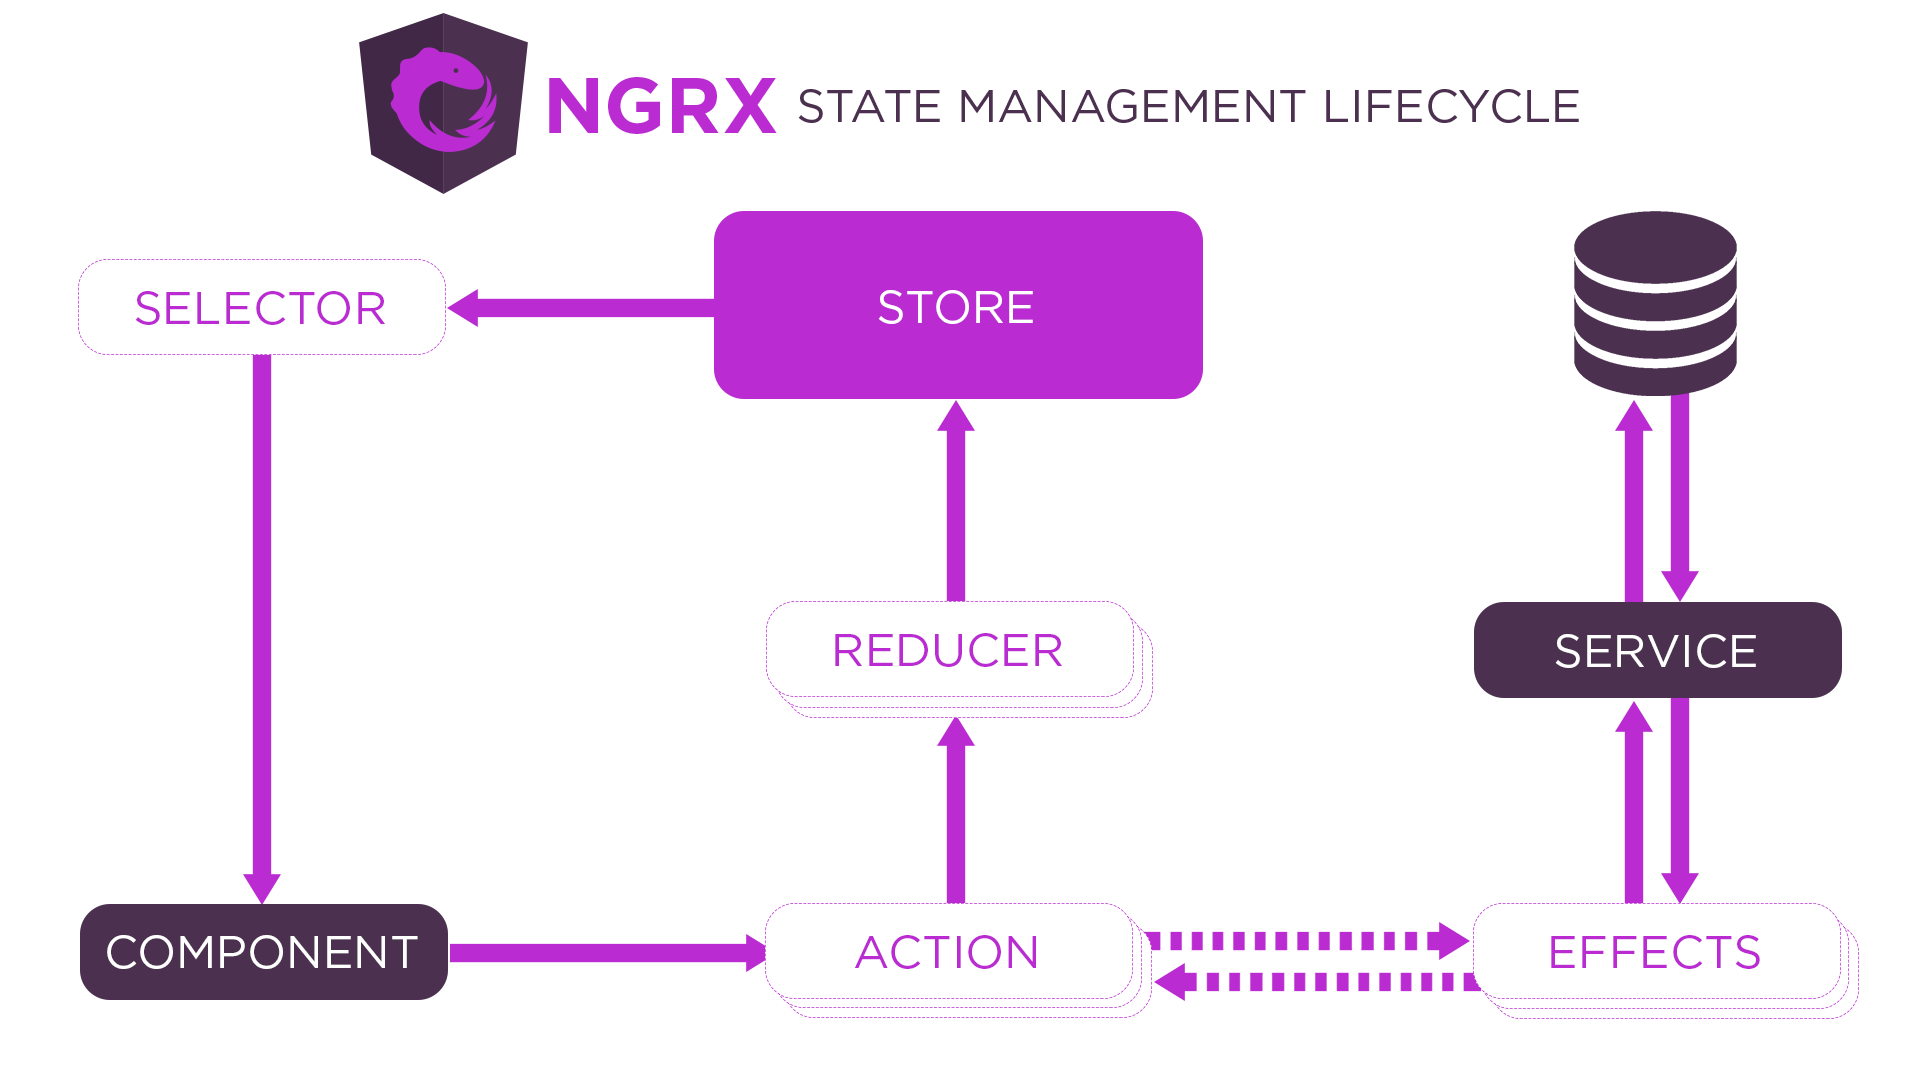
\includegraphics[width=\textwidth]{obrazky-figures/ngrx-lifecycle.png}
	\caption{Životní cyklus správy stavu s využitím knihovny NgRx. @todo popsat uzly \emph{Převzato z~\cite{bib:ngrx-lifecycle}}.}
\end{figure}
\blindtext

\subsubsection{DevExtreme}
DevExtreme je balík komponent určený pro tvorbu responzivních webových aplikací. Je k dispozici pro knihovny jQuery, Konockout, AngularJS, Angular, Vue, React, ASP.NET MVC 5 a ASP.NET Core.  
\blindtext

\section{REST}
\blindtext[2]

\section{JSON Web Token}
\emph{Tato podkapitola vychází z~\cite{bib:jwt}}

JSON Web Token (zkráceně JWT) je otevřený standard\footnote{RFC 7519: \url{https://tools.ietf.org/html/rfc7519}} zajišťující zabezpečenou výměnu informací mezi dvěma stranami. Jedná se o objekt typu JSON, který se skládá ze tří částí oddělených tečkou. Jedná se o hlavičku, náklad a podpis.

Hlavička je objekt typu JSON, zakódovaný pomocí Base64Url\footnote{Kódování reprezentující binární data pomocí tisknutelných znaků~\cite{bib:base64}} který nese informaci o typu žetonu a použitém algoritmu digitálního podpisu. 

Náklad je stejně jako hlavička objekt typu JSON zakódovaný pomocí Base64Url. Tentokrát jsou však jeho obsahem tvrzení (angl. claim). Ty nesou přenášené informace, které je třeba předávat zabezpečené. Nejčastěji se jedná o informace o uživateli.

Podpis zaručuje, že zpráva nebyla pozměněna. Může být také využit pro ověření identity odesílajícího. Podpis je vytvořen spojením řetězců dvou předchozích částí, mezi které je vložena tečka. Na konec toho řetězce je dále připojen tajný řetězec. Výsledný řetězec je poté zašifrován algoritmem uvedeným v hlavičce. 

V praxi se lze s touto metodou autentizace setkat například na stránkách, které umožňuji přihlásit se pomocí účtu u společnosti Google~\cite{bib:google-jwt}. V takovém případě se jedná o výměnu informací mezi třemi stranami. Posloupnost akcí pro získání žetonu v této situaci a jeho následné použití lze vidět na obrázku~\ref{img:jwt}.

\begin{figure}[H]
    \label{img:jwt}
	\centering
	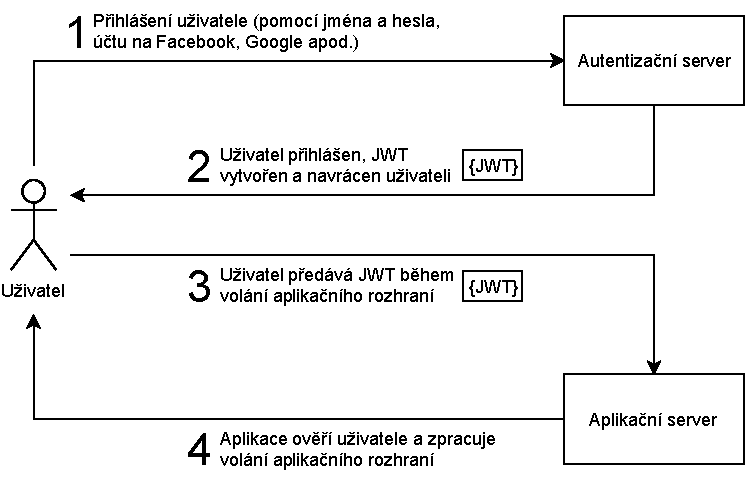
\includegraphics[width=0.9\textwidth]{obrazky-figures/jwt.pdf}
	\caption{Diagram znázorňující případ užití standardu JWT.}
\end{figure}

\section{ASP.NET Core}
ASP.NET Core je platforma společnosti Microsoft určena pro tvorbu webových aplikací. Jedná se o rozšíření populární platformy .NET určené především pro programovací jazyk C\#, taktéž vyvinutým společností Microsoft.

Přestože tato společnost stojí za dnes nejpopulárnějším operačním systémem Windows, je platformu ASP.NET Core možné provozovat i na jiných operačních systémech. Vydání první verze této platformy proběhlo v roce 2016~\cite{bib:asp-release}, dříve bylo možné platformu využít pouze na operačním systému Windows, tyto dřívější verze nesly název pouze ASP.NET bez označení Core~\cite{bib:asp-what-is}.

\blindtext

\section{PostgreSQL}
\blindtext



% ======================================================================
\chapter{Návrh aplikace}
Před samotnou implementací aplikace bylo nejprve nutné promyslet návrh aplikace. 
\blindtext


\section{Schéma systému}
Schéma aplikace je vidět na snímku~\ref{img:scheme}. Jsou zde znázorněny tři její hlavní části -- databáze, serverová část neboli SSBLite a v neposlední řadě webový klient Kanban. U každé z těchto částí je na snímku uvedena také její nejpodstatnější technologie. Dále zde lze pozorovat vzájemné interakce těchto části. Na pravé straně obrázku lze vidět dvě role uživatelů a také jejich interakci s aplikací.

\begin{figure}[H]
    \label{img:scheme}
	\centering
	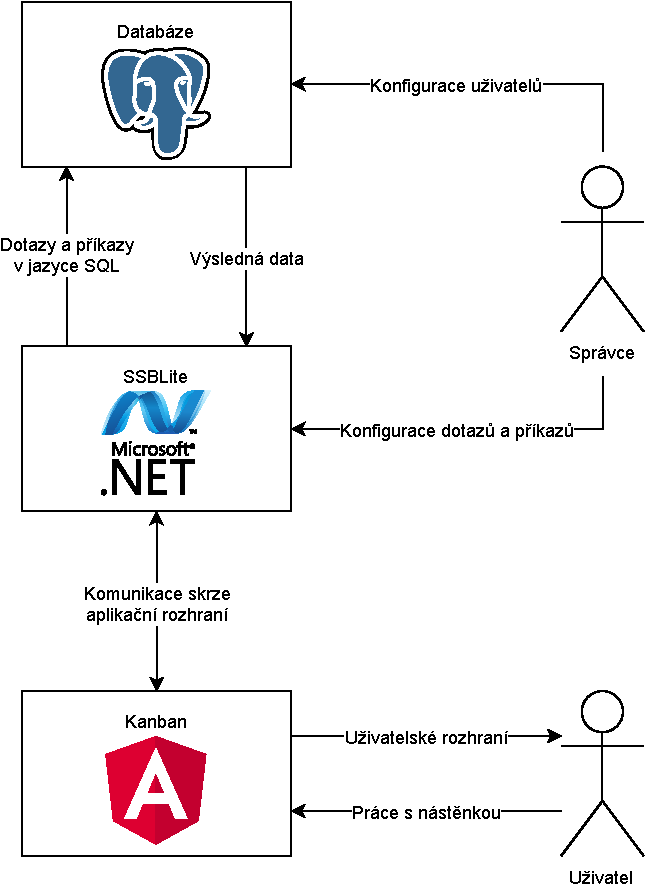
\includegraphics[width=0.8\textwidth]{obrazky-figures/app-scheme.pdf}
	\caption{Schéma vzájemných interakcí jednotlivých částí aplikace, jejich technologií a možnostech různých rolí uživatelů.}
\end{figure}

V tomto schématu se může zdát podivuhodná konfigurace uživatelé správcem přímo v databázi. V reálném prostředí, kde bude aplikace SSBLite nahrazena plnohodnotnou aplikací SSB, bude konfigurace probíhat již přímo v aplikaci SSB pomocí uživatelského rozhraní. Nicméně pro účely této bakalářské práce postačí konfigurace tímto náhradním způsobem. Vzhledem k pozdějšímu nahrazení aplikace SSBLite by implementace této funkcionality nebyla efektivní.

\section{Entitně-vztahový diagram}\label{sec:erd}
Data aplikace jsou uložena v relační databázi. Systém SSB a tedy i SSBLite využívají databázový systém PostgreSQL. Data jsou uložena v jednotlivých tabulkách, které lze reprezentovat entitně-vztahovým diagramem znázorněným na obrázku~\ref{img:erd}. Názvy tabulek i sloupců jsou dle konvence společnosti v anglickém jazyce. Tabulky ve většině případu reprezentující entity (například nástěnky, karty nebo štítky), výjimku tvoří pouze propojovací tabulky, které reprezentují vztah N ku N. Ty lze poznat podle číslovky \texttt{2} v názvu tabulky. Před a za touto číslovkou se pak nachází názvy entit, které ve vztahu figurují.

\begin{figure}[H]
	\centering
	\label{img:erd}
	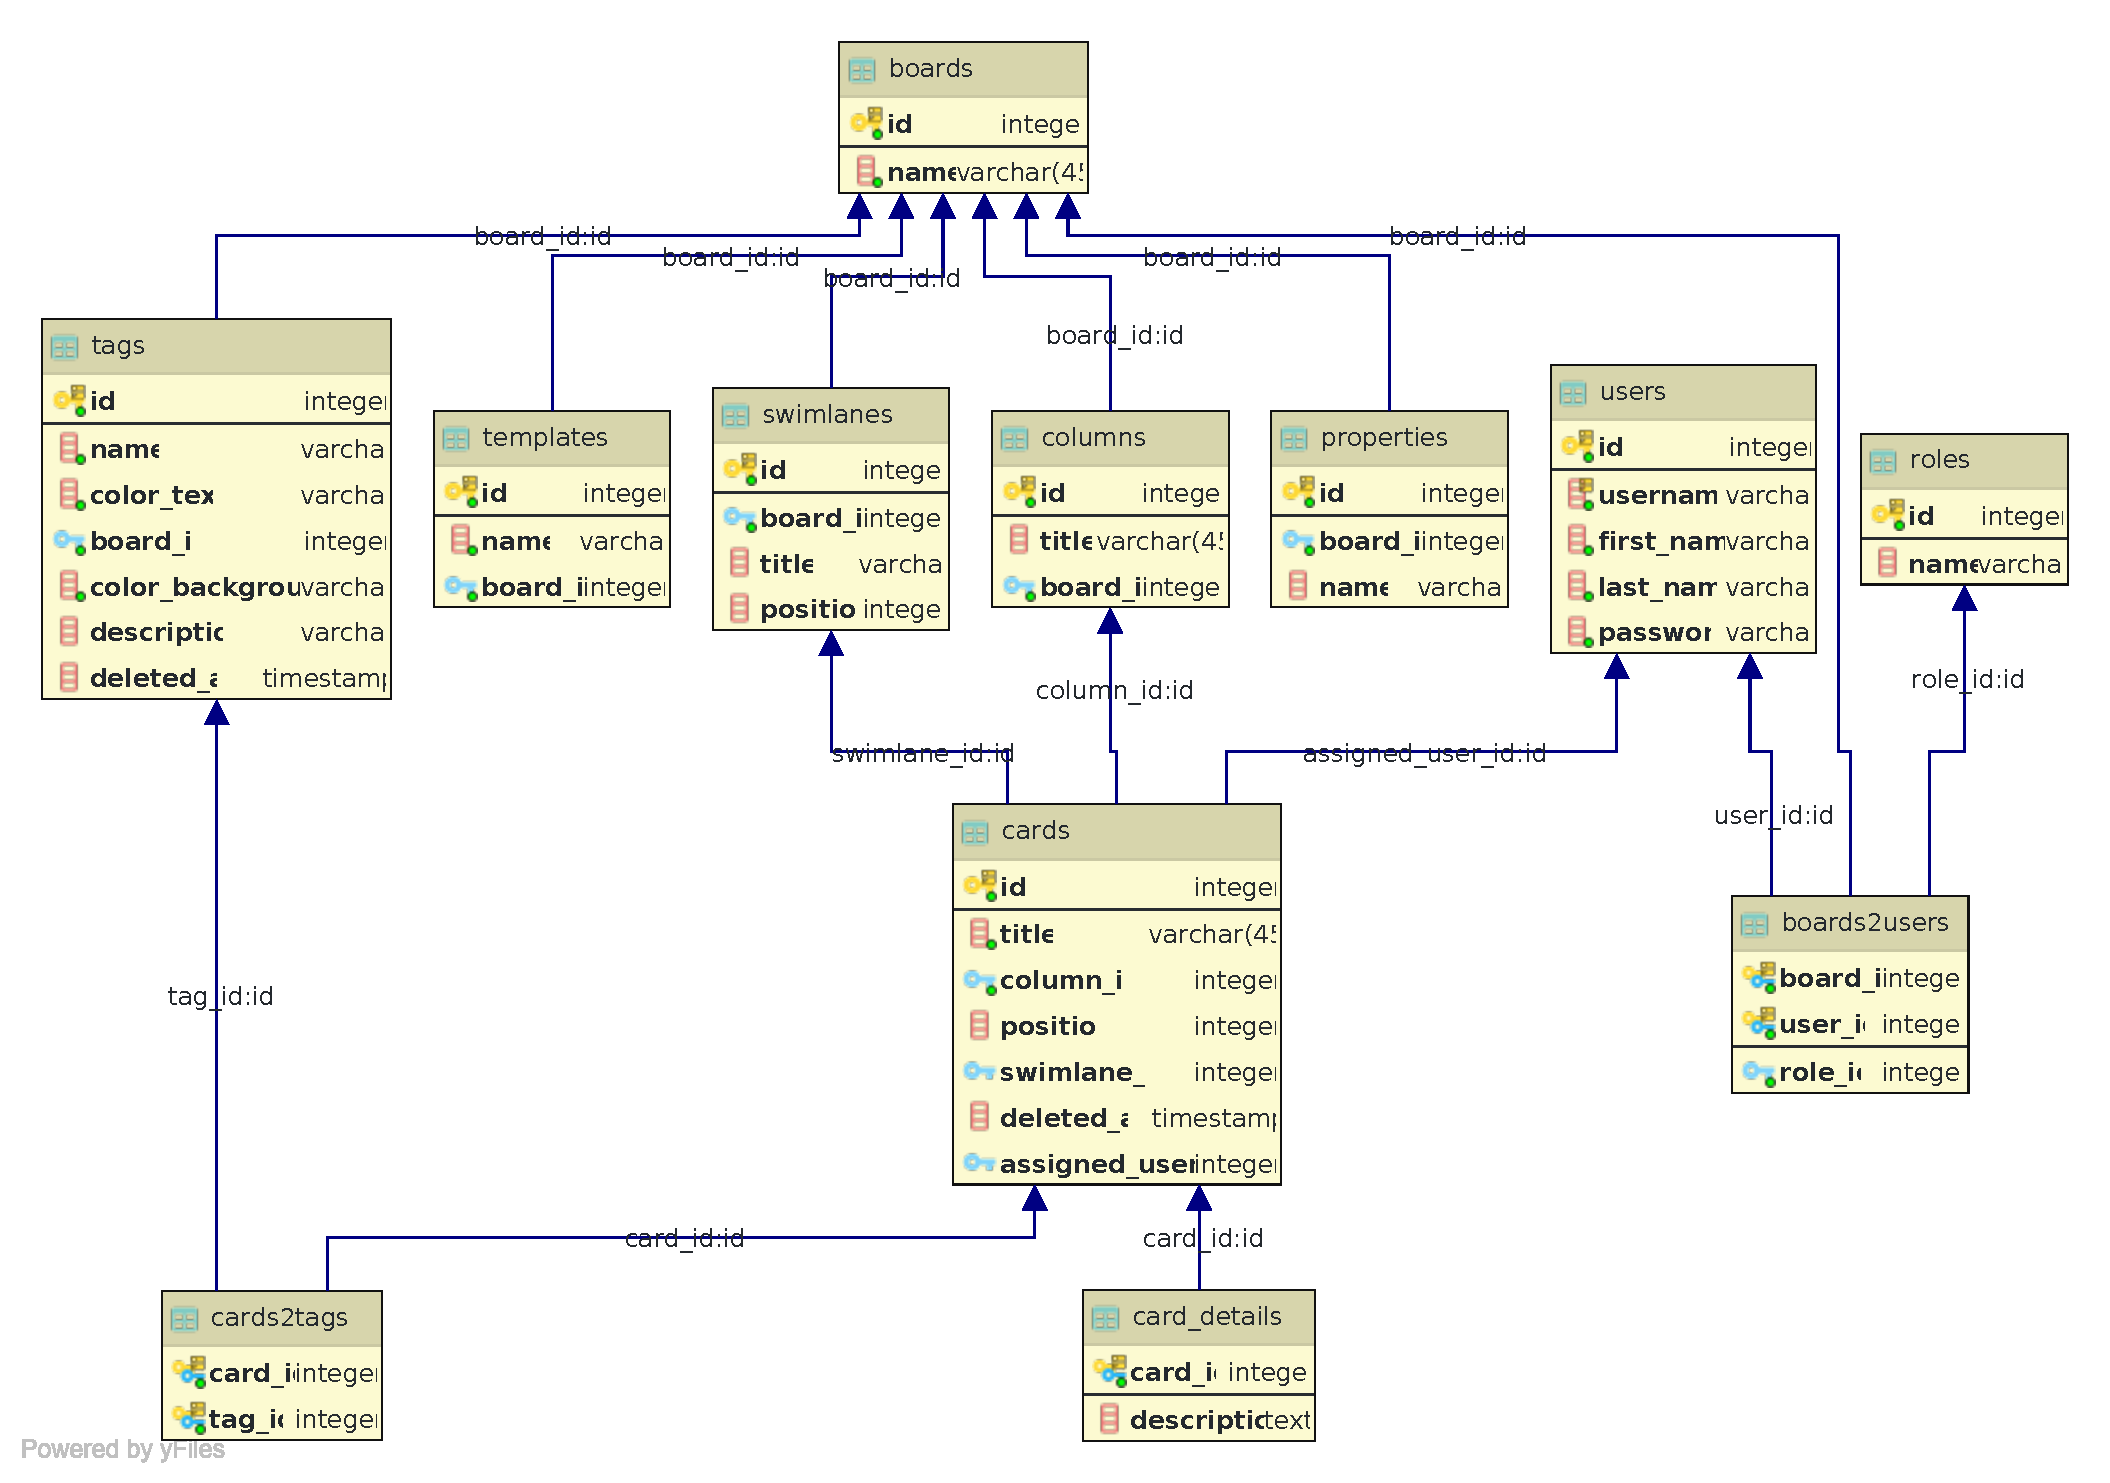
\includegraphics[width=\textwidth]{obrazky-figures/erd.pdf}
	% @todo Konverze z svg do pdf to nejak rozbila
	\caption{Entitně vztahový diagram reprezentující relační databázi aplikace.}
\end{figure}


\section{Grafický návrh}
Prvotní verze aplikace, která vznikla řešením této bakalářské práce bude využita pouze pro interní účely společnosti. Z tohoto důvodu nebyl při zadání práce kladen příliš velký důraz na estetickou stránku aplikace. Jedním z požadavků však bylo, aby aplikace co nejvíce využívala grafický styl knihovny DevExtreme. Další požadavek zněl, aby byly v aplikaci použity barvy loga společnosti SEACOMP s.r.o.

\begin{figure}[H]
	\centering
	
\includegraphics[width=\textwidth]{obrazky-figures/placeholder.pdf}
\end{figure}


\section{Aplikační rozhraní}\label{sec:api}
Komunikace mezi klientskou částí aplikace a tou serverovou probíhá za pomoci aplikačního rozhraní REST. Zprávy tohoto rozhraní využívají formát JSON a mají přesně definovaný obsah.
Vzhledem k budoucí integraci mnou tvořené aplikace do již existující aplikace SSB4Web bylo nutné zachovat v obou těchto aplikacích jednotnou podobu rozhraní.

Vzhledem k zaměření mé aplikace nebylo třeba využít všechny možnosti existujícího rozhraní. Při práci byly z původního rozhraní použity pouze dva koncové body a to \texttt{SSBQuery/GetData}, umožňující dotazovat se na data uložena v databázi, a \sloppy\texttt{SSBMethod/ExecuteMethod}, spouštějící uložené procedury či příkazy. Toto rozhraní však bylo nutné rozšířit o možnost autentizace uživatele. Pro tento účel slouží nově přidaný koncový bod \sloppy\texttt{SSBAuthentication/VerifyCredentials}.

Obě části aplikace -- jak Kanban, tak SSBLite -- využívají stejné datové objekty, díky tomu je možné mezi těmito dvěma částmi jednoduše přenášet data. Obsahem požadavku pro získání dat je například objekt \texttt{SSBQueryRequestDTO}, ten s sebou nese jednak název konkrétního před-připraveného dotazu pod klíčem \texttt{queryName} a dále pod klíčem \texttt{filters} může obsahovat i další objekt typu \texttt{SSBFilterDTO}. Ten se zase skládá z objektu \texttt{ssbIFilterOperator}, skrytým pod stejnojmenným klíčem, a dále z pole objektů \texttt{SSBFilterTermDTO} označeným klíčem \texttt{filterItems}. Objekty v tomto poli obsahují tři hodnoty. Pod klíčem \texttt{m\_filterOperator} lze opět pozorovat objekt \texttt{ssbIFilterOperator}. Ve skutečnosti se jedná pouze o výčet logických operátorů, které jsou později použity pro bezpečné sestavení dotazu na databázi. Další dvě hodnoty nesou název sloupce v databázi a pole hodnot použitých v dotazu.

Konkrétní dotaz na získání karet s použitím filtru nástěnky tak může vypadat následovně:

\begin{verbatim}
{
  "queryName": "getCards",
  "limit": 0,
  "onlyVisibleColumns": true,
  "offset": 0,
  "filter":
    {
      "ssbIFilterOperator": 0,
      "filterItems":
        [
          {
            "m_filterOperator": 0,
            "m_column": "col.board_id",
            "m_values": [1] ¨
          }
        ]
    }
}
\end{verbatim}

Nevýhoda této podoby aplikačního rozhraní je však v nemožnosti provést více dotazů na databázi pomocí jednoho asynchronního volání. Například při prvotním načtení nástěnky je tak nutné odeslat vícero asynchronních požadavků najednou.

Tento nedostatek je způsoben tím, že je původní návrh rozhraní je zaměřen hlavně na zobrazení tabulek ve vztahu hlavní--podrobné (angl. master--detail), kde k těmto situacím dochází minimálně. Zadavateli tématu diplomové práce bylo představeno několik alternativních řešení, nicméně bylo rozhodnuto pro zachování původního návrhu a setrvání v odesílání několika požadavků současně. 

https://www.overleaf.com/project/5d9f7ad34e15d80001c95e73
% ======================================================================
\chapter{Implementace aplikace}
Předmětem této kapitoly je popis vlastní implementace webové aplikace typu Kanban, která byla cílem zadání této bakalářské práce. V úvodu je popsaná klientská část aplikace, ke které uživatel přistupuje pomocí internetového prohlížeče. Další část kapitoly je věnována implementaci serverové části aplikace, s kterou uživatel přichází do styku pouze pomocí aplikačního rozhraní přiblíženého v kapitole~\ref{sec:api}. Závěr kapitoly je pak zaměřen na databázovou vrstvu aplikace, kde jsou uchovávány uživatelská a jiná data.



\section{Klientská část}
Klientskou částí aplikace je jednostránková webová aplikace vytvořená za pomocí rámce Angular. Základním stavebním kamenem toho rámce jsou bez pochyby komponenty. Právě ty jsou hlavním tématem této podkapitoly. Dále jsou zde zmíněny i jiné zajímavé části implementace klientské části. Obsah jednotlivých stránek je sestaven kombinací vlastních komponent, které jsou podrobněji popsané v této kapitole, a také před-připravených komponent knihovny DevExtreme.


\subsection{Struktura adresáře}
Adresář, ve kterém se nachází zdrojové kódy aplikace je kvůli využití rámce Angular poměrně rozsáhlá. Některé jeho části, které stojí za zmínku jsou popsány v této podkapitole. Zajímavé části nejvyšší úroveň adresáře aplikace vypadají následovně:

\begin{itemize}
  \item \texttt{node\_modules} -- Zdrojové kódy knihoven třetích stran
  \item \texttt{src} -- Zdrojové kódy aplikace
  \begin{itemize}
    \item \texttt{app} -- Adresář obsahující zdrojové kódy aplikace v jazyce TypeScript
     \item \texttt{assets} -- Adresář obsahující statický obsah stránky jako například globální kaskádové styly a obrázky
     \item \texttt{index.html} -- Hlavní stránka aplikace
  \end{itemize}
  \item \texttt{angular.json} -- Konfigurace rámce Angular
  \item \texttt{package.json} -- Konfigurace závislostí na knihovnách třetích stran
\end{itemize}

Nejdůležitějším z výše uvedených adresářů je jednoznačně adresář \texttt{app}. Pro lepší přehlednost je jeho obsah uveden zvlášť níže:

\begin{itemize}
  \item \texttt{} -- 
  \item \texttt{} --
\end{itemize}


\subsection{Základní struktura stránky}
Ať už se uživatel aktuálně nachází na libovolné části aplikace, základní struktura právě zobrazené stránky se bude tvořit ze stejných prvků. Základ celé komponenty je element \texttt{<app-root>}. Tento prvek je také kromě referencí na soubory obsahující zdrojové kódy jazyka JavaScript to jediné, co se v obsahu stránky zobrazí v případě, že internetový prohlížeč jazyk JavaScript nepodporuje či dokonce blokuje. 

V případě, že je interpret jazyka JavaScript dostupný, vzniknou uvnitř tohoto elementu další elementy. Vždy je přítomna komponenta \texttt{<app-header>} a \texttt{<router-outlet>}. První z komponent obsahuje hlavičku s logem společnosti SEACOMP s.r.o., která je vždy vidět ve vrchní části aplikace. Součástí hlavičky je také možnost odhlášení uživatele, za předpokladu že je právě přihlášen.

Druhá z komponent ve skutečnosti nemá žádný reálný obsah. Představuje však nedílnou součást aplikace, jelikož se stará právě o chování aplikace jako jednostránkové. Na základě aktuální cesty obměňuje komponentu, která v hierarchii uzlů HTML představuje dalšího sourozence. Z počátku se tak lze na tomto místě potkat s komponentou \texttt{<app-login>}, následně \texttt{<app-dashboard>} a poté \texttt{<app-board>}. Současně s obměnou těchto komponent je také změněna adresa aktuální stránky v adresním řádku internetového prohlížeče. Navenek se tedy může zdát, že uživatel skutečně přechází z jedné stránky na druhou. Ve skutečnosti se však nachází stále na stejné stránce, pouze je překreslována část jejího obsahu.

Cesty a jim odpovídající komponenty jsou definované v souboru \texttt{app-routing.module.ts}. U každé cesty je také možno nastavit ochranné služby. Jedná se o třídy implementující rozhraní \texttt{CanActivate}, které ve stejnojmenné metodě vrací logickou hodnotu. Pokud jedna z těchto služeb vrátí hodnotu nepravdy, je přístup uživatel k této cestě zamítnut. Tuto funkcionalitu v aplikaci využívám na ověření, zda je uživatel přihlášen. Výjimku tvoří pouze stránka s přihlášením, ke které lze přistoupit v přesné opačné situaci a to když uživatel zatím není přihlášen. Jedná se o třídy \texttt{AuthenticationGuardService} a \texttt{GuestGuardService}.

\begin{figure}[H]
	\centering
	
\includegraphics[width=\textwidth]{obrazky-figures/placeholder.pdf}
\end{figure}


\subsection{Nástěnka}
Stránka s nástěnkou je bezesporu nejkomplexnější částí aplikace. Její základní komponentou je <app-board>, jejím úkolem je mimo jiné také prvotní načtení všech % @todo

Na nejvyšší úrovni této stránky se nachází několik komponent knihovny DevExtreme. Jedná se o <dx-toolbar>, % @todo



\subsection{Detail karty}
\blindtext


\subsection{Nastavení}
\blindtext


\subsubsection{Nastavení štítků}
Modální okno s nastavením štítků cíleně porušuje jeden z pravidel principu Flux. Uchovává totiž lokální kopii sdílených dat uložených ve skladu. Tento přístup jsem zvolil z jednoho prostého důvodu a to aby se v případě zahození změn nemusel stav štítků napříč celou aplikací změnit. Místo toho jsem se přiklonil k opačnému řešení. Při úpravě štítků uživatel pracuje pouze s kopií sdílených dat. Jeho změny se tak neprojevují v jiných komponentách. V případě zahození změn při zavření dialogu tudíž není nutné provést vůbec žádnou akci. 


\subsection{Asynchronní požadavky}
Jak již bylo zmíněno v kapitole~\ref{sec:spa}, jednostránkové aplikace fungují hlavně díky asynchronním požadavkům. Ty jsou tedy samozřejmě nedílnou součástí i této aplikace.

Po přihlášení uživatele každý jeho asynchronní požadavek v hlavičce protokolu HTTP obsahuje žeton standardu JWT. O tuto funkci se stará třída \texttt{JwtInterceptor}, umístěná ve složce \texttt{interceptors}. Třída naslouchá všem odesílaným požadavkům protokolu HTTP a v případě, že je žeton již dostupný, je před samotným odesláním požadavku nejprve rozšířena jeho hlavička. Do pole \texttt{Authorization} je vloženo slovo \texttt{Bearer} a za mezerou následuje znění žetonu.

Ve stejné složce lze také nalézt další třídu \texttt{ErrorInterceptor}, která obstarává oznámení uživateli v případě negativní odpovědi na odeslaný požadavek. Tato třída byla užitečná obzvláště během vývoje, jelikož chyby jazyka JavaScript se zobrazují v konzoli internetového prohlížeče, tudíž nejsou na první pohled zřetelné. Nicméně tato třída přináší užitek i pro koncové uživatele ve výsledné verzi aplikace.

V případě úspěšné odpovědi na asynchronní požadavek jsou data obsažená v této zprávě uložena do skladu dat. Tento proces je podrobněji vysvětlen v následující kapitole.


\subsection{Centrální datový sklad}
Data sdílena mezi více komponentami jsou uložena v centrálním skladu, který je realizován pomocí knihovny NgRx. Při implementaci byl kladen důraz na co nejmenší zanořování dat, která jsou v tomto skladu přítomna. Každá sdílené entitě (např. nástěnkám, uživatelům, štítkům) tedy odpovídá právě jeden objekt v první úrovni zanoření.

Každý z těchto objektů je pak tvořen dalšími třemi hodnotami. Klíč \texttt{loading} obsahuje logickou hodnotu, která indikuje, zda se data právě načítají. Tato hodnota je kladná v období mezi odesláním asynchronního požadavku a přijmutím odpovědi od serveru. Uživateli tak může být dočasně skryt obsah části stránky, který čeká právě na onu odpověď. V případě kladné odpovědi jsou přijatá data převedena do vhodného tvaru a poté uložena jako pole či objekt do hodnoty označené klíčem \texttt{data}. V případě neúspěchu dotazu je pak chyba uložena do hodnoty pod klíčem \texttt{error}.

O zmíněné převedení formátu se stará třída \texttt{SSBQueryDataResultParser}. Ta převádí nevhodný tvar dat přenášených pomocí aplikačního rozhraní, kde je informace o sloupcích a datech rozdělena do dvou polí. Metoda této třídy z těchto dvou polí vytvoří jedno pole obsahující objekty, ve kterých jsou již názvy sloupců a jejich hodnoty v podobě jaká je u objektů typu JSON obvyklá.

Ani tato podoba dat však není finální. Výstupem zmíněné metody jsou totiž generické objekty. Pro veškeré přenášené entity však v aplikaci existuje odpovídající třída ve složce \texttt{models}. Generické objekty sice v aplikaci ve většině případů fungují, ale chybí jím specifické metody. V případě modelu uživatele lze například využít virtuální atribut \texttt{fullName}, který je ve skutečnosti pouze složenina dvou jiným atributů. Tento atribut by tedy v případě generického objektu dostupný nebyl. 
To je důvodem proč je využita funkce \texttt{plainToClass} knihovny \texttt{class-transformer}\footnote{Repozitář knihovny class-transformer: \url{https://github.com/typestack/class-transformer}}, která data dále převede do finální podobny.

Samotné ukládání přijatých dat a změnu obsahu skladu se zase starají reducery, které využívají zmíněnou třídu pro převod dat. 

Okamžitá vizuální odezva je však pro uživatele velmi důležitá. V některých případech je tak tedy nutné data ve skladu změnit dříve, než je přijata odpověď od serveru. Je tomu tak například u přesunu karty. Jistě by bylo pro uživatele velice nepříjemné, kdyby přesunul kartu na nové místo a ta se vzápětí ihned vrátila na svou původní pozici a až po nějaké době by akci server potvrdil a karta by se přesunula na místo, kam uživatel původně zamýšlel. Proto je v takových případech předpokládán úspěch akce a data jsou ihned změněna. I tuto práci obstarává reducer.

Pro lepší ilustraci je níže uveden snímek~\ref{img:ngrx-devtools}, který ilustruje část dat aplikace uložených právě v popisovaném centrálním skladu.

\begin{figure}[H]
	\centering
	\label{img:ngrx-devtools}
	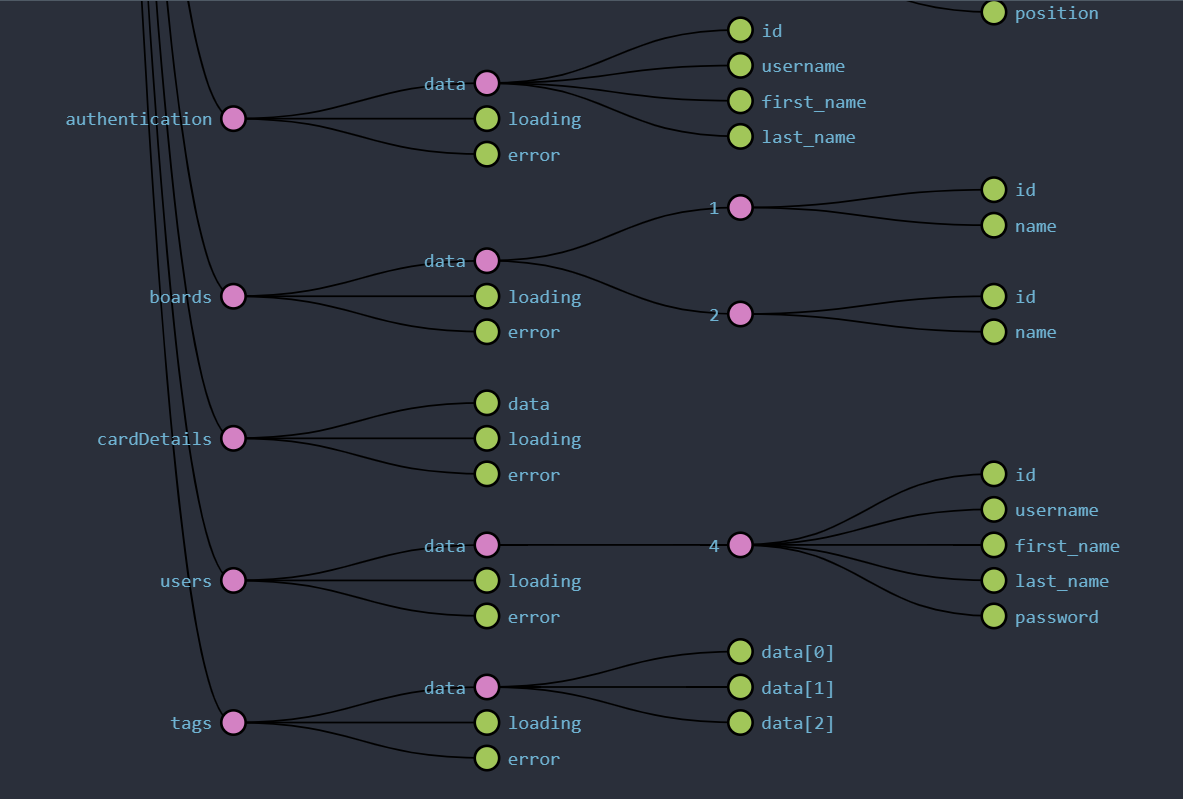
\includegraphics[width=\textwidth]{obrazky-figures/ngrx-chart.png}
	\caption{Vizualizace dat obsažených v centrálním datovém skladu. Snímek je pořízen z nástroje Redux DevTools\footnote{Redux DevTools: \url{https://chrome.google.com/webstore/detail/redux-devtools/lmhkpmbekcpmknklioeibfkpmmfibljd}}}
\end{figure}



% ======================================================================
\section{Serverová část}
Z důvodu zachování firemního tajemství klientská část mé práce nekomunikuje přímo se systémem SSB, ale pouze se zjednodušenou verzí zvanou SSBLite, kterou jsem vytvořil v rámci řešení této bakalářské práce. Jedná se o webový server vytvořený s použitím systému ASP.NET. Server zpracovává požadavky aplikačního rozhraní REST na základě kterých sestrojuje a odesílá požadavky na databázi. Výsledky těchto požadavků jsou poté odeslány zpět klientovi ke zpracování a zobrazení uživateli.

Samotný webový server neobsahuje aplikační logiku, slouží pouze jako zprostředkovatel přístupu k databázi, ke které klient z důvodu bezpečnosti nesmí mít přímý přístup. Možné požadavky na databázi jsou předem definovány a uloženy v konfiguračních souborech. Díky tomu je možné v budoucnu upravit chování aplikace bez nutnosti přímého zásahu do zdrojového kódu serverové části aplikace. 


\subsection{Struktura adresáře}
\blindtext

\begin{itemize}
  \item \texttt{Configurations/} -- Adresář obsahující konfigurační soubory metod a dotazů na databázi
  \item \texttt{Controllers/} -- 
  \item \texttt{Enums/} -- Adresář obsahující objekty výčtů, používaných aplikačním rozhraním
  \item \texttt{Helpers/} -- Adresář obsahující třídu, která umožňuje přístup k tajnému klíči aplikačního rozhraní
  \item \texttt{Interfaces/} -- % @todo
  \item \texttt{Models/} -- Adresář s třídami objektů modelů
  \begin{itemize}
    \item \texttt{Authentication/} -- 
    \item \texttt{Method/} -- 
    \item \texttt{Query/} -- 
  \end{itemize}
  \item \texttt{Services/} -- 
  \item \texttt{appsettings.json} -- 
  \item \texttt{Startup.cs} -- 
\end{itemize}


\subsection{Konfigurační soubory}
Konfigurační soubory využívají formát JSON a obsahují názvy jednotlivých požadavků a jejich znění. To však v mnoha případech přímo neobsahuje platný dotaz na databázi, ale obsažený dotaz je obohacen o klíčová slova, která umožňují přizpůsobení jeho znění pro aktuální potřebu klienta. Před samotným odesláním dotazu do databáze je nutné tyto klíčová slova zpracovat. Příkladem, využívajícím klíčové slovo \texttt{\{WHERE\}}, je následující dotaz:
\begin{verbatim}
{
    "name": "getCards",
    "content": "SELECT car.* FROM cards car JOIN columns col ON col.id = 
        car.column_id JOIN boards boa ON boa.id = col.board_id {WHERE}"
},
\end{verbatim}


\subsection{Zpracování požadavku GetData}
\blindtext


\subsection{Zpracování požadavku ExecuteMethod}
\blindtext


\subsection{Autentizace uživatele}
\blindtext



\section{Databázová vrstva}
Jak již bylo zmíněno, databáze využívá systém PostgreSQL. Ve většině podobných aplikací databáze slouží pouze pro úschovu dat. Nicméně kvůli univerzálnosti systému SSB je nutné v databázi uchovávat i aplikační logika. Toho je docíleno pomocí uložených procedur. Koncepce uložení dat v databázi byla zmíněna již v podkapitole~\ref{sec:erd}.

Jednodušší procedury jsou psány přímo v jazyce SQL a jedná se tak především o sekvenci vícero klasických příkazů, které lze spustit pomocí jednoho příkazu (spuštění uložené procedury). Tento přístup je využit například při vytvoření nového štítku, kdy je část dat uložena v tabulce \texttt{cards} a část v tabulce \texttt{card\_details}.
% @todo Overit jestli jsem to uz nezmenil

Pro komplexnější akce bylo však nutné využít jazyk PL/pgSQL\footnote{PL/pgSQL: \url{https://www.postgresql.org/docs/9.6/plpgsql.html}}. Ten umožňuje používat například funkce nebo podmínky.

Dle požadavku zadavatele práce názvy uložených procedur dodržují konvenci, kdy v první částí názvu je uvedena entita, které se daná operace týká a v druhé části je název akce. Lze se tedy setkat s názvy jako je \texttt{tags\_sync}, která synchronizuje štítky přiřazené dané kartě. 


\subsection{Synchronizace záznamů}
V aplikaci je několik situací kdy je třeba synchronizovat záznamy. Jedná se o tři akce s daty -- úprava a odstranění existujících záznamů a vytvoření nových. Tato situace nastává zejména při nastavování nástěnky. Konkrétně při nastavení sloupců, plaveckých drah, štítků a podobně. Tyto akce jsou provedeny pomoci uložených procedur \texttt{column\_sync}, \texttt{swimlane\_sync}, \texttt{tag\_sync}.

Uvnitř této procedury se však nachází pouze volání další uložené procedury a to jedné a té stejné pro všechny zmíněné procedury. Jedná se o proceduru \texttt{sync\_handler}, která umožňuje dynamicky provádět právě synchronizaci dat. Jejími parametry jsou jednak vstupní data původních procedur (identifikátor nástěnky a data k synchronizaci) a dále také specifikace nástěnky, kde jsou data uložena a sloupce, kterých se synchronizace týká.

Díky tomu je značně zredukována redundance kódu a v kombinaci s generickým komponentami klientské aplikace lze celý systém jednoduše rozšířit o nastavení dalších prvků.





% ======================================================================
\chapter{Testování a vyhodnocení}
\blindtext

Automatizované testování nebylo při práci využito. Bylo tak rozhodnuto po konzultaci jak s vedoucím tak i se zadavatelem práce. Pro ověření funkčnosti, bezpečnosti a dalších aspektů aplikačního rozhraní bylo využito manuální testování pomocí nástroje Postman\footnote{Postman: \url{https://www.postman.com}}, který slouží jako klient pro odesílání požadavků aplikačního rozhraní REST a zobrazení odpovědí na tyto požadavky.

\blindtext[3]



% ======================================================================
\chapter{Závěr}
Cílem této aplikace bylo vytvořit webovou aplikaci typu Kanban dle požadavků společnosti SEACOMP s.r.o. Tato aplikace byla úspěšně vytvořena a lze ji plnohodnotně použít pro řízení projektů, stejně tak jako po menších úpravách integrovat do stávající aplikace SSB4Web.

\blindtext

Práce pro mne měla osobní přínos především novou zkušeností s tvorbou jednostránkových aplikací, osvojením si nových rámců pro vývoj webových stránek a realizací řešení se striktními omezeními způsobu implementace.

Výsledná aplikace bude sloužit společnosti SEACOMP s.r.o. pro interní řízení vývoje softwarových produktů 

